\documentclass[11pt,a4paper]{article}
\usepackage[margin=2.25cm]{geometry}
\usepackage[T1]{fontenc}
\usepackage[utf8]{inputenc}
\usepackage{lmodern}
\usepackage{microtype}
\usepackage{enumitem}
\usepackage{graphicx}
\usepackage{booktabs}
\usepackage{array}
\usepackage[hidelinks]{hyperref}
\setlength{\parindent}{0pt}
\setlength{\parskip}{5.5pt}
\setlist[itemize]{leftmargin=1.4em,itemsep=2pt,topsep=3pt}
\newcommand{\ruletext}[1]{\begin{quote}\bfseries #1\end{quote}}
\begin{document}
{\LARGE\bfseries DDTA - Working Model Layering and Semantic Authority}\par
\vspace{4pt}
{\large\bfseries NON CANONICAL WORKING DRAFT - REVISION 1}\par
\vspace{4pt}
This document separates concerns that were previously co-located in the Decision study. The correction was triggered while regressing the facial-access example and the sixteen ThreatForge construction ADRs against Decision revision 6: rules about how tools consume a model had started to be used as if they were semantic invariants of the governed project model.

The correction does not reject the earlier representation or realization conclusions. It relocates them to the layer that actually owns them.

\section{What the DDTA metamodel is}
A governed project model is an instance of the DDTA conceptual metamodel. The conceptual metamodel defines the language in which governed project knowledge is expressed:
\begin{itemize}
\item concepts and semantic attributes;
\item semantic relations and ownership;
\item cardinalities and value domains;
\item semantic nullability/optionality;
\item invariants over one entity, a hierarchy, or the governed corpus.
\end{itemize}
For the current study this includes concepts such as Macro Requirement and Decision, their semantic fields, the MR--Decision parent relation, and invariants such as unique semantic ownership and non-redundant Decision contribution.

The conceptual metamodel does not by itself prescribe YAML syntax, Markdown heading order, validator architecture, editor implementation, similarity algorithm, or a particular tool.

\section{Four distinct layers}
\begin{verbatim}
L1  DDTA CONCEPTUAL METAMODEL
    meaning | concepts | semantic attributes | relations
    cardinalities | semantic nullability | invariants

L2  CANONICAL REPRESENTATION CONTRACT
    field presence | explicit null/empty encoding | order | headings
    containers | mirrors | YAML/Markdown mapping

L3  MODEL REALIZATION PRINCIPLES
    executable projections | validators | schemas | authoring support
    search/similarity diagnostics | derived indexes

L4  TOOL SUPPORT / CONFORMANCE MAPPING
    which DDTA contracts a tool supports, realizes, checks,
    projects or assists with
\end{verbatim}
L4 is an evaluation/support layer, not a claim that every relation named above must become a canonical metamodel relation. Its exact relation model remains deferred until the combined MR--Decision--Requirement model is available.

\begin{center}
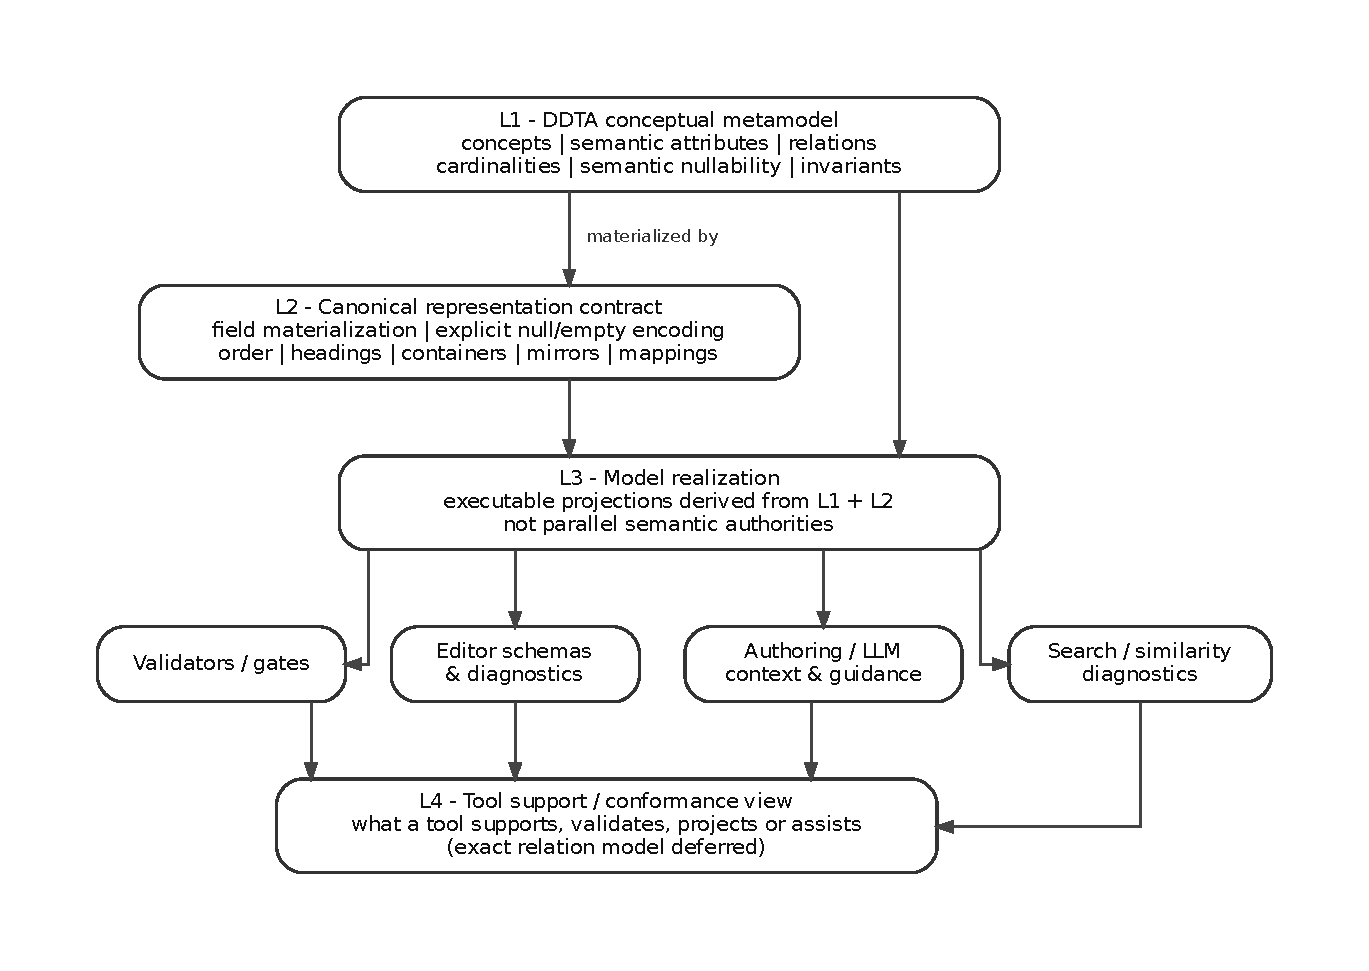
\includegraphics[width=0.96\textwidth]{diagrams/MODEL_TO_EXECUTABLE_PROJECTIONS.pdf}
\end{center}

\section{Reclassification of the Decision-study rules}
\small
\begin{tabular}{>{\raggedright\arraybackslash}p{2.8cm}>{\raggedright\arraybackslash}p{4.4cm}>{\raggedright\arraybackslash}p{7.0cm}}
\toprule
\textbf{Historical rule} & \textbf{Correct owner} & \textbf{Current interpretation}\\
\midrule
D-CLOSED-01 & L1 Decision semantics & Purpose remains Decision-specific.\\
D-CLOSED-02 & L1 Decision semantics & title/context/decision/consequences remain semantic attributes; required and non-null in the current model.\\
D-CLOSED-03 & L1 Decision semantics & Context remains decision-local.\\
D-CLOSED-04 & L1 Decision invariant & One coherent chosen position remains Decision-specific.\\
D-CLOSED-05 & L1 Decision semantics & Consequences carry material effects/trade-offs.\\
D-CLOSED-06 & Authoring/review heuristic & Useful, but not an ontological invariant. Non-goals remains outside the Decision semantic core.\\
D-CLOSED-07 & L1 Decision semantic shape & No mandatory embedded Alternatives/Rationale remains current.\\
D-CLOSED-08 & Cross-cutting L1 governance boundary & Lifecycle/status/history belong to a common governance model, not Decision-specific semantics.\\
D-CLOSED-09 & Cross-cutting semantic-authority principle & Applies across documents and tooling; not peculiar to Decision.\\
H-CLOSED-01 & L1 hierarchy invariant & Unique semantic MR ownership remains a metamodel invariant.\\
H-CLOSED-02 & L1 corpus invariant & Non-redundant Decision contribution remains a metamodel invariant.\\
R-CLOSED-01 & L2 representation contract & A canonical representation materializes every declared field.\\
R-CLOSED-02 & Split L1/L2 & Semantic nullability belongs to L1; material encoding of absence belongs to L2.\\
R-CLOSED-03 & L1--L2 boundary & Prevents syntax/layout from becoming ontology.\\
R-CLOSED-04 & L3 realization principle & Preserved, but not a semantic invariant of a governed DDTA project.\\
\bottomrule
\end{tabular}
\normalsize

Historical identifiers are retained so that the evidence sequence remains reconstructable. Relocation is not rejection of the underlying conclusion.

\section{Cross-cutting semantic authority}
\begin{verbatim}
DDTA conceptual metamodel / method
    owns portable general semantics and method-level choices

Governed project
    owns concrete governed instances and project-specific choices

ThreatForge tool
    supports authoring, resolution, validation, projection and workflow
    without becoming the semantic owner of DDTA concepts

ThreatForge project operations
    govern development of ThreatForge itself
    without becoming universal DDTA rules
\end{verbatim}
The replacement test remains useful as a review heuristic: if ThreatForge were replaced by another tool, a statement that should remain true is likely owned by DDTA or by the governed project rather than ThreatForge product architecture.

This does not imply that ThreatForge has no architectural Decisions. Once DDTA semantics are external, ThreatForge can still make genuine choices about how to support them.

\section{Canonical representation contract}
\subsection*{R-CLOSED-01 - Complete canonical shape}
Every field declared by a canonical document representation is materially present in every conforming instance representation. A missing declared field is a representation non-conformity, not an implicit semantic value.

\subsection*{R-CLOSED-02 - Semantic nullability versus material encoding}
The semantic model decides whether a value may be absent. The representation profile decides how a permitted absence is encoded.
\begin{verbatim}
semantic question:
    may assumptions have no value?                -> L1

representation question:
    when absent, is the canonical materialization
    assumptions: null or another declared form?   -> L2
\end{verbatim}
A collection may have a semantically meaningful empty set; that is distinct from an absent value. Empty string is not a generic absence marker unless a field contract explicitly gives it that meaning.

\subsection*{R-CLOSED-03 - Semantic / representation separation}
Meaning, semantic types, relations, cardinalities and invariants remain independent from physical ordering, headings, containers, mirrors and serialization mappings. A Markdown order such as Context--Decision--Consequences may be mandatory for a profile without becoming an ontological ordering relation.

\section{Model realization principles}
\subsection*{R-CLOSED-04 - Executable projections are realization, not metamodel semantics}
Validators, editor contracts, authoring assistance, machine-readable schemas and other executable consumers should derive their interpretation from the governed model and representation contracts rather than maintain independent semantic inventories.

This remains an accepted realization principle because it reduces semantic drift and enables deterministic support. It must not be used as if a governed DDTA project were semantically invalid merely because such tooling is absent.

Equally, the principle must not automatically eliminate a ThreatForge ADR. A ThreatForge Decision may legitimately choose how to realize executable contracts when multiple implementation strategies are plausible.

\section{Scalable diagnostics are tooling}
Large projects may require deterministic assistance for semantic review that is easy to perform manually in a small example. A tool may retrieve candidate overlaps or conflicts using BM25-style ranking, TF--IDF/cosine, fingerprints, term overlap, controlled-term normalization or another deterministic/indexable technique.

The metamodel owns the property to be reviewed, for example one natural MR owner or non-redundant Decision contribution. The tool only narrows the candidate set. A similarity score does not establish semantic equivalence, duplication, conflict or correct parentage. Algorithm, tokenization, weighting and thresholds remain tooling choices.

\section{Controlled vocabulary boundary}
A controlled vocabulary, if adopted, is governed knowledge rather than an implementation detail of ThreatForge. Its canonical concepts and definitions must remain meaningful if the tool is replaced. Tool mechanisms such as stemming, lexical normalization, ranking synonyms or search indexing remain L3 unless explicitly promoted into governed semantics.

The study has not yet established that every DDTA project must possess a controlled vocabulary. Its universal, optional, profile-specific or recommended status remains open.

\section{ThreatForge support / conformance view}
ThreatForge should eventually make explicit which DDTA contracts it supports without copying those contracts into its own MR/Decision prose as if it owned them.

A future support view may distinguish relations such as supports authoring for, validates structural part of, projects, assists review of, or realizes representation of. The exact canonical shape is deliberately deferred; it may ultimately live in Requirements, implementation trace, conformance evidence, or another relation model.

Example:
\begin{verbatim}
DDTA H-CLOSED-01: exactly one semantic MR parent
    -> ThreatForge may validate structural cardinality
    -> ThreatForge may assist semantic parent review

DDTA H-CLOSED-02: non-redundant Decision contribution
    -> ThreatForge may retrieve suspiciously similar Decisions
    -> governed review still decides semantic redundancy
\end{verbatim}

\section{Consequence for ThreatForge ADR regression}
A prior regression step treated R-CLOSED-04 as if it were inherited semantic truth of the DDTA metamodel and therefore used it to dismiss some ThreatForge candidate ADRs as redundant. That reasoning is withdrawn.

The correct question is:
\ruletext{Given the DDTA conceptual and representation contracts, does ThreatForge still face a meaningful choice among plausible ways to support or realize them?}
If yes, the ADR may be a legitimate ThreatForge product Decision. If no, it may instead be a Requirement, consequence, support-coverage assertion or implementation detail.

At minimum, the candidates concerning controlled-value resolution, executable document-model contracts, Security-model support and registry-derived extensibility must be re-read under this corrected layering before their Decision status is finalized.

\section{Open cross-document constraints retained}
These remain open problems for the combined governed-knowledge model rather than Decision fields or tooling algorithms:
\begin{itemize}
\item no orphan normative decision;
\item single-source governed knowledge;
\item effective governed context;
\item Decision survivability and recoverability;
\item coverage awareness for pervasive/cross-cutting obligations;
\item no inheritance-by-copy;
\item legitimate cross-MR relevance without multiple hierarchical ownership.
\end{itemize}
Their minimal semantic relation model remains deferred until Requirement semantics is studied.

\end{document}
